\documentclass[a4paper,12pt,twoside]{article}
\usepackage{fancyhdr}
\usepackage{float}
\usepackage{graphicx}
\usepackage{amsmath}
\usepackage{breqn}
%\usepackage[francais]{babel}
\usepackage[T1]{fontenc}
%\usepackage[latin1]{inputenc}
\usepackage[utf8]{inputenc}
\usepackage[alsoload=astro]{siunitx}
\usepackage[colorlinks,bookmarks=true,linkcolor=blue,urlcolor=blue, citecolor=blue]{hyperref}
\usepackage{multicol}
\usepackage{mathtools}
\usepackage{amssymb}
\usepackage[table,xcdraw]{xcolor}
\newcommand{\R}{\mathbb{R}}
\usepackage{physics}
\usepackage{url}
\usepackage[
    backend=biber,
    style=authoryear,
    natbib=true,
    url=false, 
    doi=true,
    eprint=false,
    useprefix=false,
    maxbibnames=9,
    maxcitenames=1,
    uniquelist=minyear,
    sorting=ynt
]{biblatex}
\addbibresource{refs.bib}
\usepackage[left=2cm, right=2cm, top=1cm, bottom=1.5cm, headheight=25pt, includehead, headsep=44pt]{geometry}
\usepackage{multicol}
\usepackage{color}
%\pagestyle{plain}

%Pour changer la taille des titres de section et subsection. Ajoutez manuellement les autres styles si besoin.
\makeatletter
\renewcommand{\section}{\@startsection {section}{1}{\z@}%
             {-3.5ex \@plus -1ex \@minus -.2ex}%
             {2.3ex \@plus.2ex}%
             {\normalfont\large\bfseries}}
\makeatother

\makeatletter
\renewcommand{\subsection}{\@startsection {subsection}{1}{\z@}%
             {-3.5ex \@plus -1ex \@minus -.2ex}%
             {2.3ex \@plus.2ex}%
             {\normalfont\normalsize\bfseries}}
\makeatother

\pagestyle{fancy}
\fancyhf{}
\rhead{
\includegraphics[scale=0.09]{EPFL_Logo_Digital_RGB_PROD.png}}
\lhead{\leftmark}
\rfoot{\thepage}
\DeclareSIUnit\year{yr}
\DeclareSIUnit\h{\mathnormal{h}}

\renewbibmacro*{begentry}{\midsentence}
\newcommand{\hlight}[1]{(\color{red}#1\color{black}) }

\makeatletter
\AtBeginDocument{\toggletrue{blx@useprefix}}
\makeatother

\title{\Huge{\textbf{BAO measurement and cosmological parameter constraints using eBOSS galaxies and voids}}}
\date{\today}
\author{Daniel Felipe Forero Sánchez\\{\small \href{mailto:daniel.forerosanchez@epfl.ch}{daniel.forerosanchez@epfl.ch}} 
	\vspace{7mm} \\ Supervisor: Cheng Zhao \vspace{4mm} \\ Professor: Jean-Paul Kneib}


\begin{document}


\maketitle
\baselineskip=16pt
\parindent=15pt
\parskip=5pt
\vspace{1 cm}

\section*{Abstract}
Baryon Acoustic Oscillations (BAO) are a signal imprinted in the 3-dimensional distribution of various tracers in the Universe. It provides a standard scale that can be measured at different redshifts. In the present work, we aim to use the eBOSS survey ELG tracers and the large ($R>\SI{16}{\h^{-1} \mega\parsec}$) cosmic voids  to  measure the BAO scale in the redshift range of $0.6<z<1.1$. Nonetheless, the observed BAO signal obtained from the voids is not significant enough for it to improve the measurement that can be obtained from the galaxy BAO. Additionally, the two-point correlation functions show unaccounted for systematical effects in the survey. These are more prominent in the galaxy and small void ($R<\SI{8}{\h^{-1} \mega\parsec}$) distributions, than they are in the large voids'.
%TODO add more lines for people not necessarily in the field

\newpage

\tableofcontents

\newpage
\sisetup{separate-uncertainty = true,
        bracket-numbers=true}
\section{Introduction}
Baryon Acoustic Oscillations (BAO) provide a \textit{standard ruler} or scale that can be tracked at different redshifts, its measurement is then of This is due to the fact that it allows us to further improve the constraints on cosmological parameters \citep{Bassett2010}. The signal is encoded in the spatial distribution of matter in the Universe. Traditionally, different kinds of massive cosmic objects or \textit{tracers}, as well as the anisotropies in the Cosmic Microwave Background (CMB) are used to measure the scale. This work aims towards the measurement of the BAO peak by combining Emission Line Galaxies (ELG) and the voids in their distribution (see section \ref{sec:voids}), following previous work by \textcite{Zhao2019}.\\
In section \ref{sec:theory} we discuss the basics of the BAO phenomenon and the use of cosmic voids as tracers of under-densities. Section \ref{sec:method} discusses the method used to analyze the data, including the software to generate the void catalogs from a given galaxy one. Then, section in section \ref{sec:results} we show the obtained results for different tracers, while in section \ref{sec:discussion} we discuss them. Finally, we state the conclusions of the study and mention some future directions.

\section{Background theory\label{sec:theory}}
\subsection{Baryon Acoustic Oscillations}
Nowadays, the baryonic matter of the Universe can be roughly distributed in a 75\% hydrogen and a 25\% helium. Nevertheless, before we had these elements, in the early Universe, the temperature was high enough for the protons and electrons to be found separately: at this stage we had an ionized plasma. The components of this plasma were electrically charged, thus, electromagnetically interacting with the photon gas, whose short mean free path made the Universe optically thick. In addition to the ionized plasma, dark matter was also present at these early stage. \\
The behavior of small matter density anomalies $\delta$ is described by equation \ref{eq:inhom}. Notice that it has the form of an oscillator. These are what we call \textit{Baryon acoustic oscillations} (BAO). These are entirely dependent on the coupling between baryonic matter and photons.
\begin{equation}
    \Ddot{\delta} + 2H\Dot{\delta} + \qty{\frac{c_s^2k^2}{a^2}-4\pi G\rho}\delta = 0
    \label{eq:inhom}
\end{equation}
Notice the factor in braces has a \textit{pressure term} $\qty(\frac{c_s^2k^2}{a^2})$ and a \textit{gravitational term}, $\qty(4\pi G\rho)$. The oscillatory behavior is expected as long as $\frac{c_s^2k^2}{a^2}>4\pi G\rho$. This inequality also holds without gravity, however, its presence implies that the oscillations will be dampened and that if $k= a\frac{\sqrt{4\pi G\rho}}{c_s}\equiv k_J$ (Jeans' wavenumber), the oscillation frequency would be zero. This tells us that at small scales ($k>k_J$), pressure dominates and drives the oscillatory behavior, while at large scales ($k<k_J$), the gravitational term will dominate and fluctuations will simply grow \citep{Baumann}.\\
Additionally, it is imperative that the baryonic plasma is coupled (electromagnetically) to the photon gas for this process to be carried on. Therefore, this phenomenon will stop happening when such coupling disappears. This happens at the age of recombination, when the hydrogen is formed (and not destroyed by high-energy photons) and the baryonic gas becomes neutral, hence, transparent to the photons. This, in turn, implies that these oscillations were ``frozen'' at time $t_{rec}\approx\SI{4e5}{\year}$, while the previously decoupled photon gas was free to leave, forming the CMB. This, rather well-known time, combined with the speed at which this pressure waves moved, can be used to define a \textit{standard ruler} or a characteristic scale \citep{Eisenstein1997, Eisenstein2007}, that is, a standard angular distance that can be accurately measured at different redshifts.\\
It is possible to compute the distance at which these oscillations were frozen, a.k.a. the \textit{sound horizon}, more formally defined as the comoving distance the sound waves travel from $t=0$ to $t=t_{rec}$ \citep{Weinberg2013}. This quantity can be easily computed knowing that the comoving distance travelled with speed $c_s$ is
\begin{equation}
    \chi_s = \int_{0}^{t_{rec}}\frac{c_s(t)}{a(t)}\dd t.
\end{equation}
In our case, $c_s = c/\sqrt{3(1+R)}$ with $R\equiv 3\rho_b/\rho_\gamma$ \citep{Eisenstein1997, Dodelson2003} and the result is $\chi_s \approx \SI{150}{\mega\parsec}$ \citep{Weinberg2013}.
Once the photon gas decoupled, the remaining BAO peak continued to interact gravitationally with the dark matter, so we expect the latter to also show such characteristic, see figure 1 in \textcite{Eisenstein2007}.\\
Then, this BAO signature is imprinted both in the characteristic size of the temperature anomalies of the CMB and in the clustering of galaxies. The analysis of the former yields values of $\chi_s(z_{rec}) = \SI{ 146.8 \pm 1.8}{\mega\parsec}$ and $\chi_s(z_{drag}) = \SI{ 153.3 \pm 2.0}{\mega\parsec}$ \citep{Komatsu2009}. In the latter case, the sound horizon can be statistically extracted from the 3D distribution of galaxies by means of the \textit{two-point correlation function} (2PCF), this is, the histogram of the separations between a pair of galaxies \citep{Peebles1980,Eisenstein2005}. A nice illustration can be found in figure 1.5 of \textcite{Bassett2010}, alongside a thorough explanation on how the signal is encoded in the tracer distribution.\\
As explained before, the BAO phenomenon, and the signal, is inherent to the matter distribution in the Universe. This means that a variety of different tracers can be used to extract the signal. This is rather convenient when looking for it at different redshifts. Some previously used tracers are quasars \citep{McDonald2007, Ata2018}, galaxies \citep{Eisenstein2005} and galaxy clusters \citep{Hong2012, Hong2016}. Recent studies \citep{Kitaura2016, Liang2016, Zhao2019} evaluate the possibility to use cosmic voids as tracers, too.


\subsection{Voids\label{sec:voids}}
Given that the BAO signal is encoded in the distribution of galaxies or \textit{matter tracers}, we can expect to be able to get information from the distribution of the underdensities or \textit{voids}. However, the definition of voids is rather difficult and depends strongly on the matter tracer used \citep{VandeWeygaert2009}. The many possible definitions of this kind of structure has produced different kinds of void-finding algorithms. As stated by \textcite{Zhao2016}, we can outline some common definitions of voids as follows.\\ \textcite{Colberg2005} define voids as regions with mean overdensity of at most $-0.8$. Such regions are minima of the smoothed initial density field, where spheres are located and subsequently merged according to a set of rules (see reference for details) to form the final voids. A second approach is that of \textcite{Hahn2007, Forero-Romero2009}, in which the definition of void is given by the local gravitational evolution as given by halo dynamics. \textcite{Abel2012} analyze the cosmic web in phase space and classify regions according to the DM stream density. Voids are defined as particles that record being part of only their primordial stream (see figure 5, top-left panel in the reference). Finally, voids can be regarded as simply the empty regions in the spatial distribution of tracers. Among these, the first three depend on free parameters such as the smoothing scale of the density field \citep{Hahn2007}. Either way, all definitions agree on voids being underdensities. It is this what makes them less vulnerable to non-linearities in the gravitational evolution of the Universe \citep{VandeWeygaert2009, Zhao2016}. \\
\subsection{Systematical Effects}
\color{red}SEE WHICH IS THE PAPER THAT DESCRIBES THESE, INFO TAKEN FROM THE README MEANWHILE\color{black}
\subsubsection{Fiber collisions}
For the targets' spectra to be observed, each should be assigned a fiber. When two targets are too close (less than $r_{cp}\equiv62''$), they can't be observed by the same plate, at the same time. In this case, only one of them is selected for measurement, however, the others' spectra could be measured by another plate. \hlight{NOT SURE IF THIS DEFINITION IS NECESSARY} The \textit{tiling success rate} (TSR), defined over each sector as the number of measured targets over the number of targets quantifies this effect.  \hlight{PUT TSR PLOT AS EXAMPLES?}\\
Collision groups are defined as \hlight{ARNAUD} sets of targets within the fiber collision radius, $r_{cp}$ that couldn't be observed by any plate. The \textit{close-pair weight}, $w_{cp}$ is defined (per collision group) as the total number of targets over the number of observed ones. By applying this weight to the resolved objects, unobserved targets are accounted for in the final catalog.
\subsubsection{Redshift Failures}
The success rate of the spectroscopy pipeline (SSR) is not 100\%. It can be affected by factors such as observation conditions and position of the fiber in the focal plane. \hlight{Arnaud} defines the redshift failure weight, $w_{noz}$ to take into account both these effects by estimating the SSR based on the median signal to noise ratio, $\mathrm{SSR}_{\mathrm{obs}}$, and the position in the focal plane $\mathrm{SSR}_{\mathrm{pos}}$. In this way, $$w_{noz}\equiv \qty(\mathrm{SSR}_{\mathrm{obs}}\mathrm{SSR}_{\mathrm{pos}})^{-1}.$$

\subsubsection{Angular photometric systematics}
Various effects are grouped under this category. Each is represented in a \textsc{Healpix} map by the galactic extinction, \textsc{H i} column density, Gaia stellar density, DECaLS depth and seeing parameters, hereon $p_i$. A multilinear fit to the model $$y^k = \epsilon + \sum_i c_ip_i^k$$ is performed for all $p_i^k$ using a squared error loss. The fit is done per chunk in the survey, this is eboss21, eboss22, eboss23 and eboss25. The first two are the SGC, while the other are in  the NGC. The index $k$ then labels the pixels in the chunk.\\
The weights designed to partially correct for these effects are defined as $$w_{\mathrm{systot}} = \qty(y^k)^{-1}.$$

\subsubsection{Normalization and FKP weights}
To effectively apply the weights, the mean of $w_{\mathrm{systot}}$ over all ELG objects in the chunk is normalized to one.\\
The completeness weights are then computed as
$$w_{\mathrm{comp}} = w_{\mathrm{systot}}w_{cp}w_{noz}.$$
The redshift failure weight is normalized too, such that the mean of $w_{\mathrm{comp}}$ over objects with reliable spectroscopic measurement and stars (with $w_{noz}=1$) is the same as the mean of $w_{\mathrm{comp}}$ over valid ELGs.\\
Invalid objects such as those with no reliable redshift or with a collided fiber are zero-weighted by setting $w_{noz}=0$ and $w_{cp}$ respectively.\\
The final clustering sample is obtained after selecting objects with $\mathrm{SSR}\geq0$, $z\in(0.6, 1.1)$ and completeness (number of resolved fibers over number of objects, per sector) greater than 50\%.\\
Due to the dependence of the tracer number density $n(z)$ on the redshift, we must apply too a final weight $$w_{\mathrm{FKP}} \equiv \frac{1}{1 + n(z) P_0};\quad P_0 = \SI{4000}{\h^{-3}\mega\parsec\cubic}.$$
\subsubsection{Applying systematic weights}
Through the application of the weighing schemes previously mentioned, we are able to control the systematic effects present in the final catalog. To partially apply systematics we proceed as follows:
\begin{itemize}
	\item We compute $w_{\mathrm{comp}}^{\textsc{allsyst}} =w_{\mathrm{systot}}w_{cp}w_{noz}w_{\mathrm{FKP}}$ and the effective number of tracers in each chunk $$n_{eff} = \sum_{i=1}^{N_{chunk}}w_{\mathrm{comp},i}^{\textsc{allsyst}},$$ where $N_{chunk}$ is the number of tracers in the chunk considered.
	\item We then compute $$w_{\mathrm{comp}}^{\textsc{partial}}=w_{\mathrm{FKP}}\prod_{s\in \mathcal{S}'}w_s,$$ where $\mathcal{S}' \subseteq \mathcal{S}$ is the subset of systematic effects to be considered and $\mathcal{S} =\qty{\mathrm{systot},\ noz,\ cp}$. In this case we compute the new effective number of tracers $$n'_{eff} = \sum_{i=1}^{N_{chunk}}w_{\mathrm{comp},i}^{\textsc{partial}}.$$
	\item Objects in the catalog with $w_{\mathrm{comp}}^{\textsc{partial}}=0$ or $\mathtt{veto}=0$ are removed. \hlight{ADD SECTION ON VETO MASKS?}
	\item We then normalize the completeness weights in each chunk by the corresponding $n_{eff}/n'_{eff}$ to conserve the original effective number of tracers and avoid recomputing $n(z)$.
\end{itemize}

The study of systematic effects is relevant because it has been observed that voids are less sensitive to them \citep{Kitaura2016, Liang2016}, thus potentially helping in the improvement of constraints on the cosmological parameters currently determined from the matter tracer distribution.\\
Following the work in \textcite{Zhao2016}, the present work uses the \textsc{Dive} code to generate void catalogs from a discrete set of matter tracers.
\subsection{\textsc{DIVE}}
The \textsc{Dive} code is based on the Delaunay Triangulation (DT) algorithm \citep{Delaunay1934}, that divides the space in simplices and defines voids as the circumspheres within, which do not contain tracers \citep{Zhao2016}. The code returns a void catalog, composed of the comoving coordinates of the centers of the voids and the respective radii. Additionally, the efficiency allows for an easy scaling to a large number of galaxy catalogs, for instance, mock catalogs from simulations. This is useful for estimating the covariance matrices of clustering measurements. Unlike some of the methods briefly presented in the previous section, this approach does not depend on free parameters. This code is also convenient for the study of voids as tracers, since the output is a large catalog of void-centers that favors the statistical analysis of the population.
\subsection{Types of voids}
A study \citep{Zhao2016} of the properties of DT voids, shows that the resulting catalog can be divided in two subsamples, according to the response of the number of voids in each category to the number of haloes. In particular, small spheres ($R<\SI{8 }{\h^{-1}\mega\parsec}$) are correlated to the population of haloes, while big voids seem anticorrelated. The former are called \textit{voids-in-clouds} due to their presence where matter density is higher, while on the other hand, big voids are called \textit{voids-in-voids} since they are predominantly in empty regions of the cosmic web \citep{Sheth2003}. \\
Studies on the use of cosmic voids as tracers of under-densities for BAO peak detection \citep[see][]{Liang2016} have reached the conclusion that the \textit{signal-to-noise ratio} (SNR) is maximized, in LRG (see section \ref{sec:survey}) voids, for a radius cut of $R \approx \SI{16}{\h^{-1} \mega\parsec}$. \\
Moreover, the number density of big voids has been shown to be independent on the galaxy density \citep{Kitaura2016, Zhao2016}, which has the most significant impact on the BAO measurements as shown by \textcite{Ross2017a}. On the contrary, small voids, seem to provide redundant information on the galaxy distribution, given that they are mostly located in high matter density regions \citep{Kitaura2016}. 
\subsection{The eBOSS survey\label{sec:survey}}
The Extended Baryon Oscillation Spectroscopic Survey (eBOSS) started taking data in 2014, aiming towards a precise measurement of the BAO signal from various different matter tracers such as \textit{Luminous Red Galaxies} (LRG), \textit{Emission Line Galaxies} (ELG) and \textit{Quasi-Stellar Objects} (QSO). These allow for the exploration of redshifts $z\in (0.6, 2.2)$ \citep{Dawson2015}.\\
The redshift coverage in the survey is divided as follows: LRG targets cover $z \in (0.6, 1)$, ELGs cover $z \in (0.6, 1.1)$ with 300 plates and QSO targets cover $z \in(0.8, 2.2)$. Observations are expected to take a similar time to complete as the BOSS, about 5400$~$hr \citep{Dawson2015}.\\
This work relies on the ELG part of the survey, whose redshift distribution is shown in figure AXAXZZX
Notice that small voids are distributed around the peaks of the galaxy distribution, as would be expected since these are hidden within the cosmic clouds hence the name voids-in-clouds. On the contrary, the distribution of big voids has a valley around this maximum, this shows that this type of void is located in the emptier regions of the cosmic web. The shaded regions show the $1\sigma$ band provided by the 500 mock realizations used; which seem to be in good agreement with the observations.\\
As discussed in \textcite{Raichoor2017}, the target selection is dependent on some systematic effects such as stellar density, galactic extinction, or fiber collisions. Figure ASDASDS shows the geometry of the NGC zone of the survey.

\section{Method\label{sec:method}}

As mentioned before, this work uses ELG tracers: 87585 in the North Galactic Cap (NGC), and 109537 in the SGC. However, this dataset only accounts for a single realization of the Universe. It is then necessary to study a large number of mock datasets for each of these zones in order to estimate the covariance matrix. Ideally, the number of mocks should be significantly larger than the number of data points in the observed set, however, in this work we use 500 of these realizations. Each mock must share the properties of the observational data, such as geometry of the survey and galaxy density, as well as consistent clustering statistics.\\
\subsection{Pipeline\label{sec:pipeline}}
For the observed dataset the pipeline is rather simple. The catalogs, given in sky coordinates (RA, DEC, $z$), are converted into comoving (X, Y, Z) ones. Then, \textsc{Dive} is able to find the voids, resulting in a void catalog that contains the position (X, Y, Z) of the void center and its radius $R$. in order to compute the 2PCF, it is necessary to have a random catalog, though, for the case of voids this has to be created following the procedure described in \textcite{Liang2016}.\\
On the other hand, for the mocks, the process is similar yet more time-consuming, given the large volume of data to process. In both cases, once \textsc{Dive} is done generating the void catalogs, they should be converted to sky coordinates in order to apply the appropriate masks. To do this more efficiently, we tried to combine all catalogs into a single one, thus avoiding the repetitive and time-expensive reading of the masks for each mock. Once the voids inside the survey region were selected, we could generate the random void catalog in the following way, as sketched in \textcite{Liang2016}:
\begin{enumerate}
    \item Combine 100 mock void catalogs for each zone.
    \item Divide each file in $z$-bins with boundaries 0.6, 0.7, 0.8, 0.9, 1 , 1.1.
    \item Divide each of the $z$-bins into R-bins with linearly spaced boundaries from 0 to $\SI{21}{\h^{-1}\mega\parsec}$ and bin size of 1. The last three bins are taken from 21 to 25, 25 to 30 and 30 to $\SI{50}{\h^{-1}\mega\parsec}$.
    \item Now, divide each of the resulting bins in two, one containing the RA, DEC and the other containing the $z$, $R$ columns.
    \item Shuffle in-place, the lines of one of the two halves.
    \item Undo all the splitting, that is, combine the halves, then the R-bins and then the Z-bins.
    \item Finally randomly choose some lines of the big random catalog left. In this case, We chose \num{2700000}. When choosing lines we perform the radius cut, choosing objects with $R\in (R_c, \SI{50}{\h^{-1}\mega\parsec})$, with $R_c=\SI{15.5}{\h^{-1}\mega\parsec}$ (see section \ref{sec:snr}).
\end{enumerate}
Now, with the random catalog built, it is possible to compute the 2PCFs for voids. In order to do this, we use the Landy-Szalay estimator \citep{Landy1993}
\begin{equation}
\xi = \frac{DD - 2DR + RR}{RR}.\label{eq:LSestimator}
\end{equation}
When we consider the combined galaxy and void sample, this estimator conserves the form \ref{eq:LSestimator}, however, each term has to be recomputed to account for both types of tracers as follows \citep{Zhao2019}
\begin{align}
DD &= \frac{D_gD_gn_g^2 + 2D_gD_vn_gn_vw + D_vD_vn_v^2w^2}{(n_g+n_vw)^2},\\
DR &= \frac{D_gR_gn_g^2+D_vR_vn_v^2w^2 + (D_gR_v+D_vR_g)n_gn_vw}{(n_g+n_vw)^2},\\
RR &= \frac{R_gR_gn_g^2 + 2R_gR_vn_gn_vw + R_vR_vn_v^2w^2}{(n_g+n_vw)^2}.
\end{align}
The new $w$ parameter is introduced to prevent the negative BAO peak coming from the void-galaxy cross correlation 2PCF to weaken the galaxy BAO signal \citep{Zhao2019}. 
As described in \textcite{Liang2016}, \textcite{Zhao2016} and \textcite{Zhao2019} and mentioned earlier in this text, there are two types of DT voids, we will use $R_{big} > \SI{16}{\h^{-1}\mega\parsec}$ and $R_{small} < \SI{8}{\h^{-1}\mega\parsec}$. The latter are clearly voids in the geometrical sense, nonetheless, the local dark matter density contrast around them shows that these are actually rich in dark matter, while big voids are restricted to low local DM density contrast regions \citep[see figure 9 in][]{Zhao2016}. These two cases should therefore be analyzed independently.
\subsection{SNR analysis for BAO feature\label{sec:snr}}
In order to construct the void catalogs, we analyzed the Signal-to-noise ratio (SNR) of the BAO feature in the 2PCF. To do this, we followed the work done by \textcite{Liang2016}. To be precise, we generated 100 correlation functions for the catalogs with no systematics and computed the signal $S$ defined as
\begin{equation}
S = \xi_0(s^{\mathrm{BAO}}) - \frac{\xi_0(s_1^{\mathrm{dl}}) + \xi_0(s_2^{\mathrm{dl}}) + \xi_0(s_1^{\mathrm{dr}}) +  \xi_0(s_2^{\mathrm{dr}})}{4},
\end{equation}
where we have used $s_1^{\mathrm{BAO}} = 102.5$, $s_1^{\mathrm{dl}} = 82.5$, $s_2^{\mathrm{dl}}=87.5$, $s_1^{\mathrm{dr}} = 117.5$ and $s_2^{\mathrm{dr}}=\SI{122.5}{\h^{-1}\mega\parsec}$ as originally done by \textcite{Liang2016}. The location of these points can be seen in figure \ref{fig:snrpoints}.
\begin{figure}
	\centering
	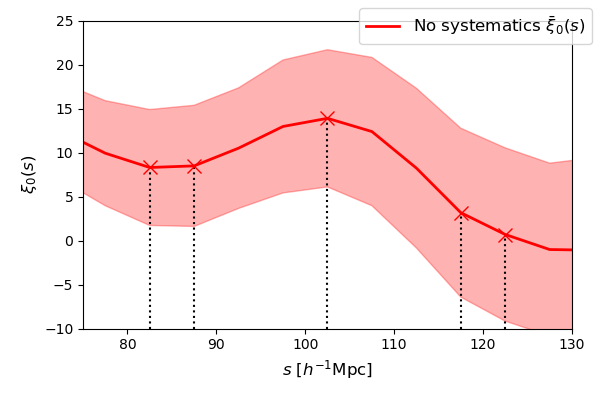
\includegraphics[width=0.7\linewidth]{plots/snr_points}
	\caption{BAO feature on the mean of the 2PCF of mocks with no systematics along with the standard deviation (shaded region). Vertical lines show the values of $s_1^{\mathrm{dl}} = 82.5$, $s_2^{\mathrm{dl}}=87.5$, $s_1^{\mathrm{BAO}} = 102.5$, $s_1^{\mathrm{dr}} = 117.5$ and $s_2^{\mathrm{dr}}=\SI{122.5}{\h^{-1}\mega\parsec}$ respectively from left to right.}
	\label{fig:snrpoints}
\end{figure}
The SNR is then
\begin{equation}
\mathrm{SNR}(R_c) = \frac{\langle S \rangle}{\sigma_S},
\end{equation}
with $\langle S \rangle$ the average signal over the 100 mocks used and $\sigma_S$ the corresponding standard deviation. We did the test for different values of the low radius cut $R_c$. Figure \ref{fig:snr} shows that the SNR peaks at $R_c =\SI{15.5}{\h^{-1}\mega\parsec}$. Note that this is different from the optimal radius-cut given by the analysis by \textcite{Liang2016}. Their SNR was also much higher, with a maximum at $\mathrm{SNR}\sim\num{e1}$.
\begin{figure}
	\centering
	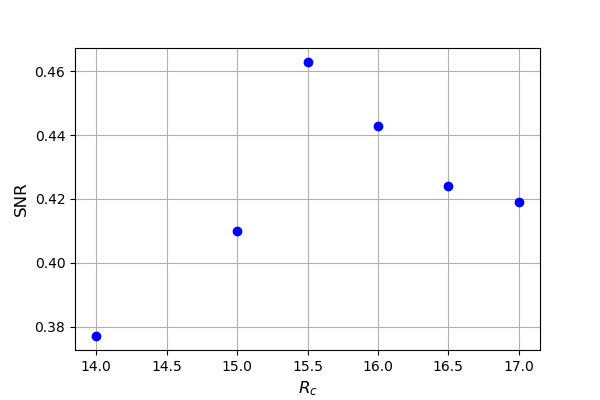
\includegraphics[width=0.7\linewidth]{plots/snr}
	\caption{SNR vs low radius cut $R_c$. Upper cut is always set to $\SI{50}{\h^{-1}\mega\parsec}$. Maximum SNR is obtained for $R_c = \SI{15.5}{\h^{-1}\mega\parsec}$.}
	\label{fig:snr}
\end{figure}

\subsection{Fitting procedure}
\subsubsection{The model}
In section \ref{sec:pipeline} we briefly outlined the necessary steps to generate the masked mock catalogs which include, for instance, coordinate conversions and computing distances. For these, a \textit{fiducial cosmology} is necessary. The introduction of this cosmology implies that our measurements depend on it in such a way that we will actually look at how the BAO feature behaves in our data with respect to what is expected from the fiducial cosmology.\\
To fit the BAO feature we use the model proposed by \textcite{Xu2012} to compute the 2PCF of the fiducial cosmology, $\xi_t$. This model relies on a generated template power spectrum, $P_{t}(k)$, which is then related to the model 2PCF via Fourier transform. As was done in \textcite{Zhao2019}, we include a Gaussian damping such that the model correlation function is
\begin{equation}
\xi_t(s) = \int\frac{k^2\dd k}{2\pi^2}\frac{\sin ks}{ks}P_t(k)\exp(-k^2a^2),
\end{equation}
where the parameter $a = \SI{1}{\h^{-1}\mega\parsec}$ \citep{Xu2012, Zhao2019}. The function $P_t(k)$ is the template power spectrum. It is obtained via the relation
\begin{equation}
P_t(k) = \qty[P_{\mathrm{lin}}(k) - P_{\mathrm{nw}}(k)]\exp\qty(\frac{-\Sigma_{\mathrm{nl}}^2k^2}{2}) + P_{\mathrm{nw}}(k).
\label{eq:pkt}
\end{equation}
The linear power spectrum $P_{\mathrm{lin}}$ is generated by CAMB software\footnote{\url{https://camb.info/}}, while the \textit{non-wiggle} power spectrum is computed from the baryonless transfer function as shown by \textcite{Eisenstein1997}. The first term in equation \ref{eq:pkt} describes the Gaussian dampening of the BAO feature (the \textit{wiggles}) while the second term just reconstructs the power spectrum with the dampening taken into account.\\
Given that $\xi_t$ describes the clustering of the fiducial cosmology, to perform our measurements we introduce the \textit{model} 2PCF,
\begin{equation}
\xi_{\mathrm{model}}(s) \equiv B^2 \xi_t(\alpha s) + A(s),
\end{equation}
which is the curve that should actually fit our data, given that it contains the parameters $B$ and $\alpha$ along with the \textit{nuisance parameters}, $a_i,\ i=1, 2, 3$ contained in the polynomial
\begin{equation}
A(s) = \frac{a_1}{s^2} + \frac{a_2}{s} + a_3,
\end{equation}
meant to fit the broadband spectrum of the data \citep{Zhao2019}. The other free parameters in the model are then $B$, for normalization, $\Sigma_{\mathrm{nl}}$ to account for the dampening of the BAO peak; and $\alpha$, the dilation parameter. The latter contains the information on how the peak is shifted with respect to the fiducial cosmology used to build $\xi_t$.\\
Nonetheless, to fit voids it is necessary to modify this model. \textcite{Zhao2019} found that the ratio between the tracer and linear non-wiggled power spectra showed a nontrivial behavior in the case of voids, while for galaxies it was almost flat. The non-linear behavior of such quantity is modeled by them as an extra quadratic term in $k$. The modified template spectrum is
\begin{equation}
P_t^v(k) = \qty{\qty[P_{\mathrm{lin}}(k) - P_{\mathrm{nw}}(k)]\exp\qty(\frac{-\Sigma_{\mathrm{nl}}^2k^2}{2}) + P_{\mathrm{nw}}(k)}\qty{1+ck^2},
\label{eq:pktmod}
\end{equation}
where $c$ is a seventh free parameter for the void fit.
\subsubsection{Parameter inference}
\section{Results}
\subsection{ELG}
\section{Conclusion}

\clearpage
\addcontentsline{toc}{section}{References}
\printbibliography[sorting=nty]
\section*{Appendix}
\subsection*{ELG tracer density distributions}

\end{document}
